\usetikzlibrary{arrows, automata, positioning}
\begin{figure}[h!]
    \begin{minipage}{0.24\textwidth}
    \scalebox{0.7}{
    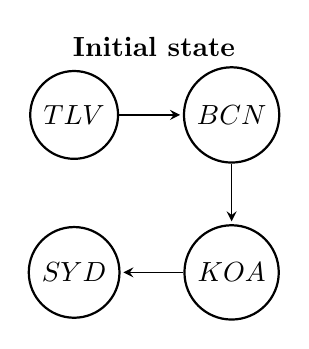
\begin{tikzpicture}[
            > = stealth, % arrow head style
            shorten > = 1pt, % don't touch arrow head to node
            auto,
            node distance = 2cm, % distance between nodes
            semithick % line style
        ]
    
        \tikzstyle{every state}=[
            draw = black,
            thick,
            fill = white,
            minimum size = 4mm
        ]
    
        \node[state] (TLV) {$TLV$};
        \node[state] (BCN) [right of=TLV] {$BCN$};
        \node[state] (KOA) [below  of=BCN] {$KOA$};
        \node[state] (SYD) [below of=TLV] {$SYD$};
        \path[->] (TLV) [] edge node { } (BCN);
        \path[->] (BCN) [] edge node { } (KOA);
        \path[->] (KOA) [] edge node { } (SYD);
    \node[above,font=\bfseries] at (current bounding box.north) {Initial state\\};
    \end{tikzpicture}}
    \end{minipage}
    \begin{minipage}{0.24\textwidth}
    \scalebox{0.7}{
    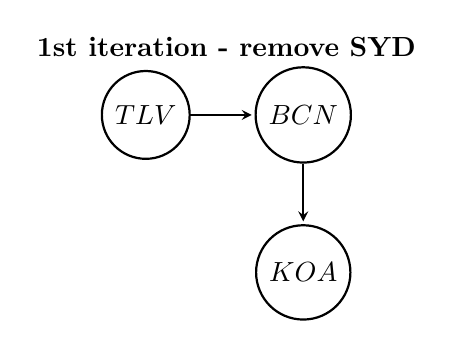
\begin{tikzpicture}[
            > = stealth, % arrow head style
            shorten > = 1pt, % don't touch arrow head to node
            auto,
            node distance = 2cm, % distance between nodes
            semithick % line style
        ]
    
        \tikzstyle{every state}=[
            draw = black,
            thick,
            fill = white,
            minimum size = 4mm
        ]
    
        \node[state] (TLV) {$TLV$};
        \node[state] (BCN) [right of=TLV] {$BCN$};
        \node[state] (KOA) [below  of=BCN] {$KOA$};
        
        \path[->] (TLV) [] edge node { } (BCN);
        \path[->] (BCN) [] edge node { } (KOA);
        \node[above,font=\bfseries] at (current bounding box.north) {1st iteration - remove SYD};
    \end{tikzpicture}
    }
    \vfill
    \end{minipage}
    \begin{minipage}{0.24\textwidth}
    \scalebox{0.7}{
    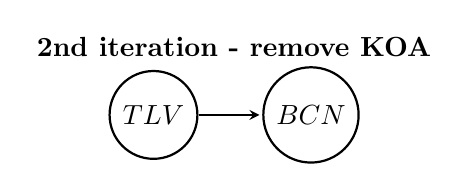
\begin{tikzpicture}[
            > = stealth, % arrow head style
            shorten > = 1pt, % don't touch arrow head to node
            auto,
            node distance = 2cm, % distance between nodes
            semithick % line style
        ]
    
        \tikzstyle{every state}=[
            draw = black,
            thick,
            fill = white,
            minimum size = 4mm
        ]
    
        \node[state] (TLV) {$TLV$};
        \node[state] (BCN) [right of=TLV] {$BCN$};
        
        \path[->] (TLV) [] edge node { } (BCN);
                \node[above,font=\bfseries] at (current bounding box.north) {2nd iteration - remove KOA};
    \end{tikzpicture}}
    \end{minipage}
    \begin{minipage}{0.24\textwidth}
    \scalebox{0.7}{
    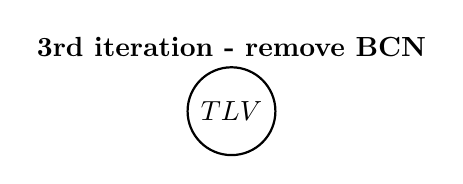
\begin{tikzpicture}[
            > = stealth, % arrow head style
            shorten > = 1pt, % don't touch arrow head to node
            auto,
            node distance = 2cm, % distance between nodes
            semithick % line style
        ]
    
        \tikzstyle{every state}=[
            draw = black,
            thick,
            fill = white,
            minimum size = 4mm
        ]
        \node[state] (TLV) {$TLV$};
        \node[above,font=\bfseries] at (current bounding box.north) {3rd iteration - remove BCN};
    \end{tikzpicture}
    }
    \end{minipage}
    \caption{1st approach}
    \label{graph:s0}
\end{figure}


